\chapter{Pacemaker} \label{chap:pacemaker}
\section{Case Description}
This model represents a pacemaker, which is a device surgically
implanted into patients at risk of certain life-threatening
irregularities developing in their heart.  A pacemaker has the task of
monitoring the heart's behaviour, and taking action if necessary to
ensure that a regular heart rate is maintained.

A human heart is divided into four chambers: at the top of the heart
are two smaller chambers: the left and right atria; and at the bottom
of the heart are two larger chambers: the left and right ventricles.
Each chamber is made of a wall of cardiac muscle fibres that contract
and then relax many times per minute.  The contractions force blood
currently inside the chamber outwards (via blood vessels).  The
subsequent relaxation of the muscle fibres allows more blood to
enter.  This maintains the regular movement of blood around the body,
and the rate and regularity with which the cardiac muscles contract
and expand is therefore very important for cardiac health.
\begin{figure}[!ht]
\centering
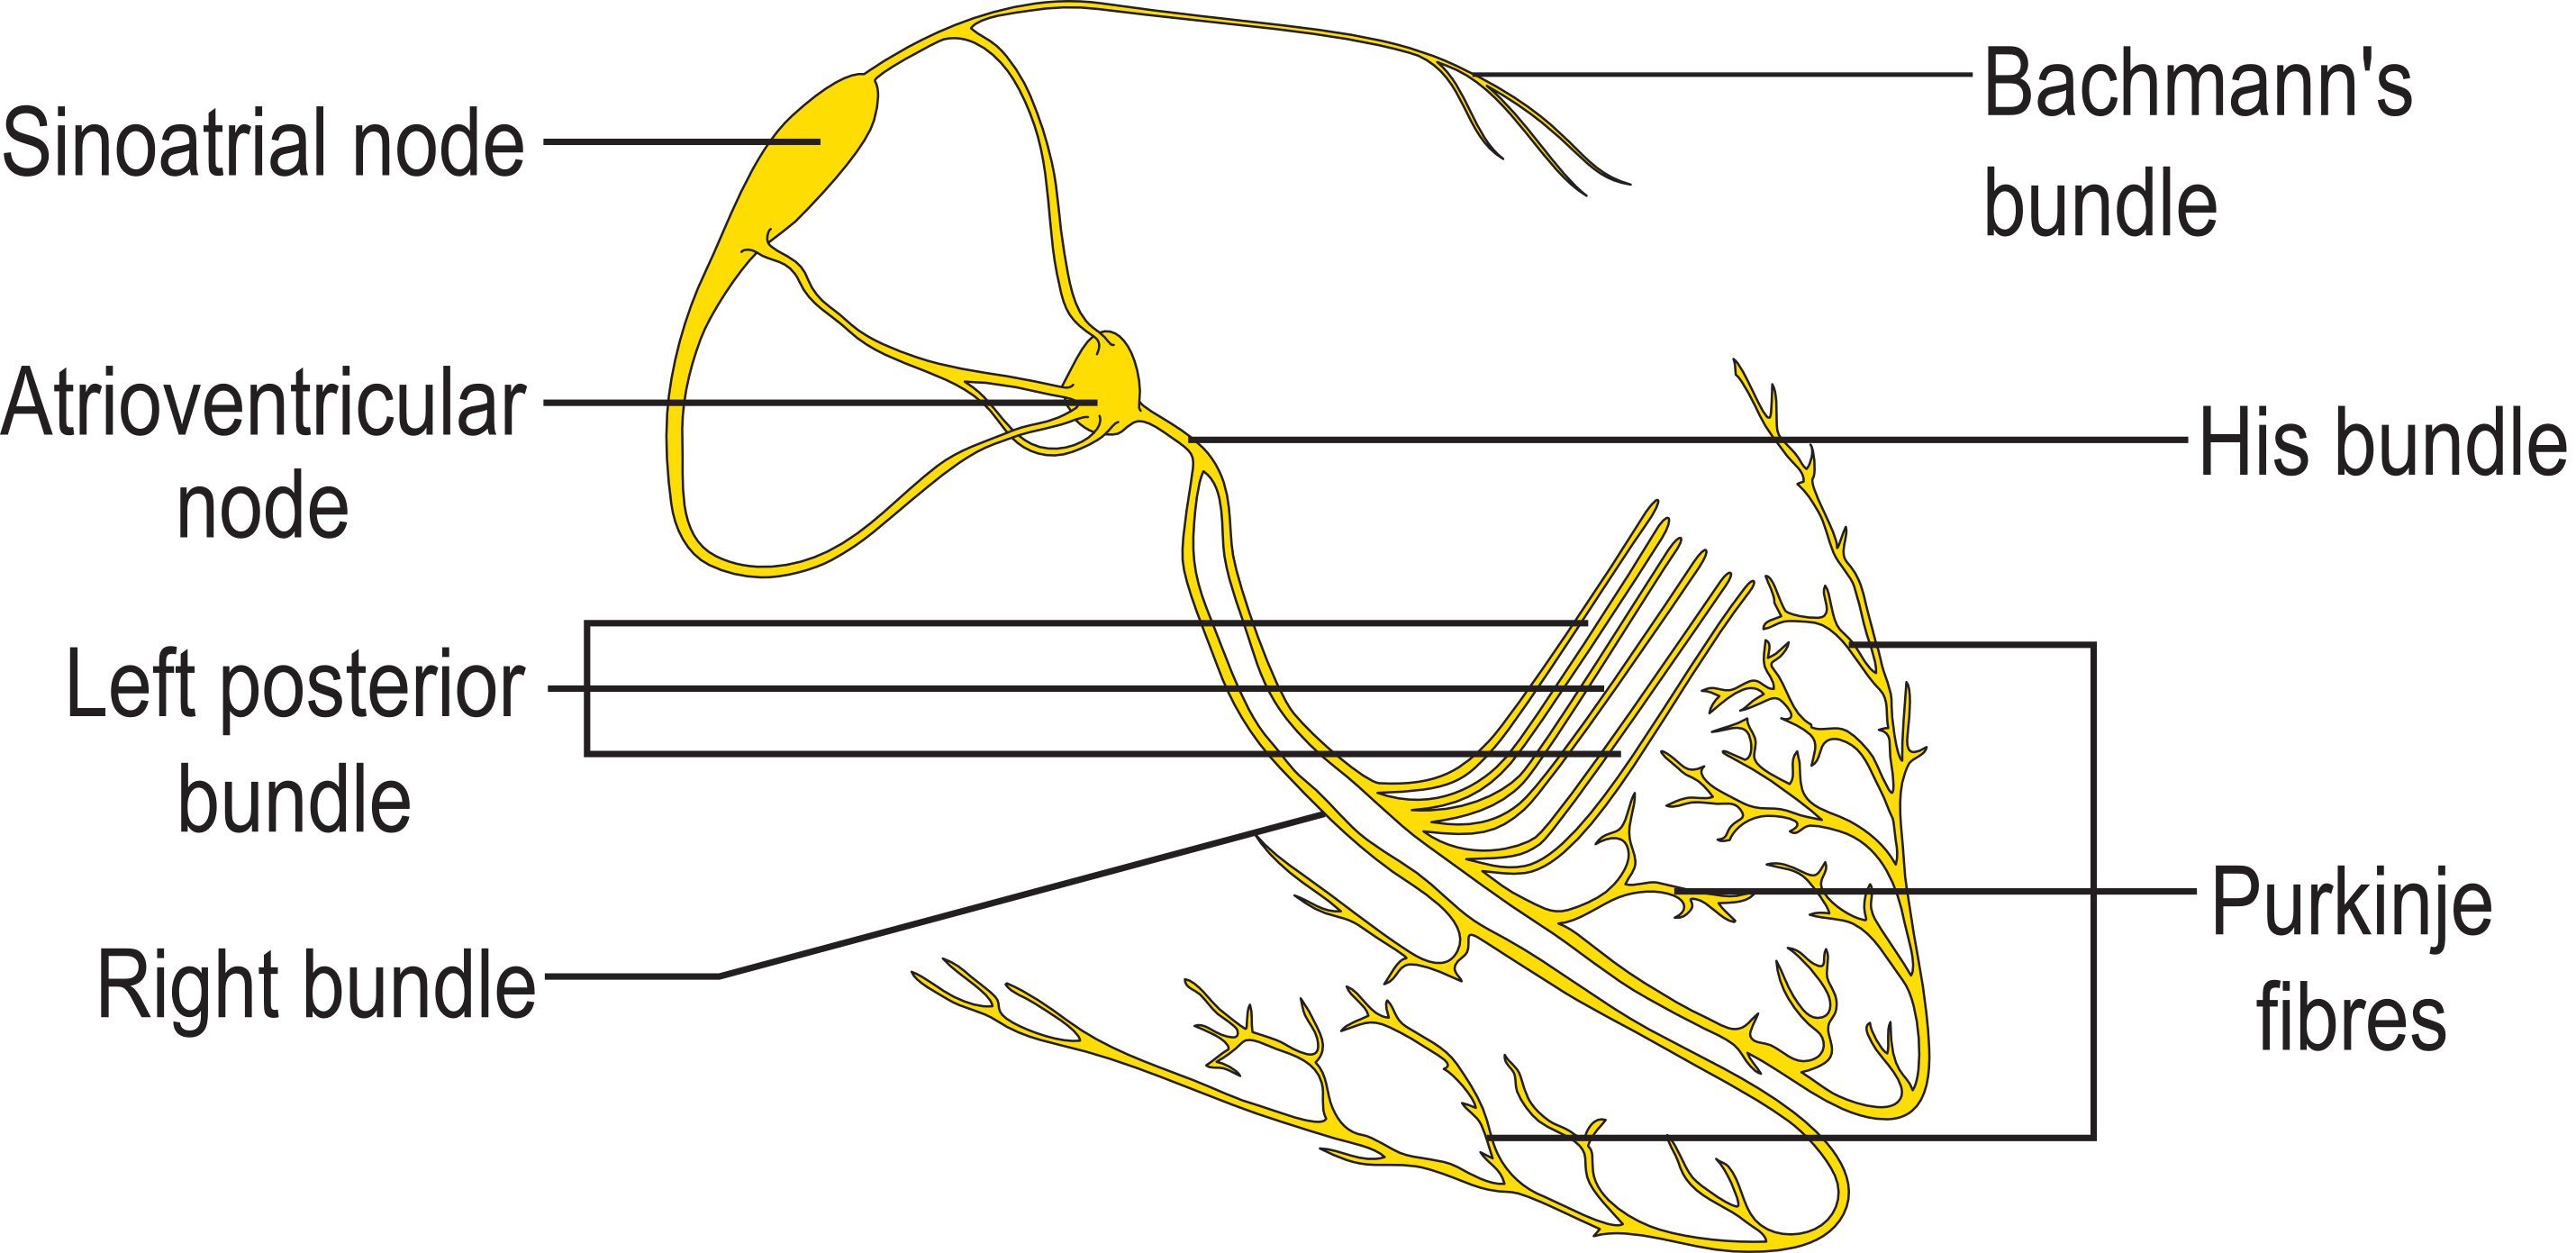
\includegraphics[width=8.5cm]{pacemaker/ConductionsystemoftheheartwithouttheHeart.png}
\caption{Electrical system of the heart.  Source:\\
  http://http://en.wikipedia.org/wiki/File:ConductionsystemoftheheartwithouttheHeart.png \label{fig:heart}}
\end{figure}

Figure \ref{fig:heart} shows the layout of the electrical system of
the heart.  The contraction of the cardiac muscle fibres is triggered
by an electrical discharge which is produced by a sinoatrial (SA)
node, situated above the atria, and by a second node, the
atrioventricular (AV) node, which is located between the atria and the
ventricles.  The two nodes are connected via a set of pathways.  A
healthy heart normally produces, in a single cycle, an electrical
discharge from the SA node, followed by a short pause, and a similar
discharge from the AV node.  This causes a regular pumping motion,
with the atria contracting and disgorging blood, then expanding just
in time to accept the blood being disgorged from the ventricles as
they contract in their turn.

A real heart is very complex and the co-model provided here
necessarily simplifies it.  In the DESTECS co-model, we represent the
heart's electrical system primarily as an SA node, an AV node and
pathways between them.  An electrical charge builds in the model
representation of the SA node over a period of time until it reaches a
threshold when it discharges quickly.  This discharge would be
absorbed into the muscle fibres surrounding the atria, and would cause
them to contract.  In the model the AV node also builds up an
electrical charge over a period of time; this charge includes some of
the charge communicated from the SA node via the pathways.  When the
AV node reaches its own threshold, it, too, discharges its electrical
charge.  This would cause the cardiac muscles in the walls of the
ventricles to contract in turn.

In a real heart, each of the two nodes has a natural rhythm for
discharging current.  The SA node tends to discharge approximately
70-100 times per minute in an average adult, and the AV node
approximately 40-60 times per minute.  In practice, however, the two
discharges in a healthy heart are synchronised and occur at the pace
dictated by the SA node.  In the co-model, this also happens; the
current discharged by the SA node is absorbed by the AV node, causing
it to reach its own discharge threshold more promptly that otherwise.

The pacemaker co-model implements a simplified version of the
behaviour of a healthy heart as described above, and also models two
well-known irregular behaviours, (there are many possible heart
irregularities we could model).  The two that we model are:

\begin{itemize}
\item \emph{Sino bradycardia}, a condition in which the SA node
  located at the top of the heart discharges too slowly.
\item \emph{Third degree atrioventricular block}, a condition in which
  the pathways connecting the two nodes fail to function properly.  Without communication between the nodes, the AV node tends to revert to
  its own, slower rhythm, and the atria and ventricles begin to lose
  their synchronisation.  The heart's efficient pumping action is thus
  compromised.
\end{itemize}

The pacemaker device has the task of monitoring the heart rate, and
when it detects that there is a problem it delivers an electrical
current to the cardiac muscle to force contractions at an appropriate
pace.  It does this only until the heart recovers and is able to
self-regulate once again, and so the pacemaker needs to monitor the
cardiac fibres continuously whilst delivering the necessary current to
regulate heart behaviour.  The pacemaker is usually connected to the
heart muscle by several electrical leads.  In this co-model, the
pacemaker itself is represented as a DE model, whilst the heart (i.e.,
the pacemaker's environment) is represented as a CT model.  The CT
model aims to model the electrical currents in the heart, and does not
model cardiac muscle fibres itself.

\section{External Links}
The pacemaker is described in the paper \cite{Gamble&12}, presented at
the Workshop on Trustworthy Cyber-Physical Systems.

\section{Contract} The contract for the pacemaker co-model contains
four variables of type \keyw{real}.  Two \emph{monitored} variables,
\texttt{atrial\_sensed} and \texttt{ventricular\_sensed}, represent
input from the sensor that detects whether the cardiac fibres in the
atria and the ventricles respectively have contracted.  And two
\emph{controlled} variables, \texttt{atrial\_paced} and
\texttt{ventricular\_paced}, deliver an electric current to the
cardiac fibres of the atria and the ventricles respectively, to force
them to contract.

\section{Discrete-event} The DE model contains a
\texttt{Controller} class which has the main thread of control.  The
\texttt{System} class creates a \texttt{Controller}, two instances of
the \texttt{ISensorReal} abstract class to represent the sensors which
monitor the cardiac muscle, and two instances of
\texttt{IActuatorReal} to represent the two leads that produce an
electric current for the muscle cells.  At runtime a concrete
implementation of the \texttt{ISensorReal} is provided by the
\texttt{Sensor} class, and a concrete implementation of
\texttt{IActuatorReal} is provided by \texttt{Actuator}.
\texttt{Actuator} simply handles the passing of a signal to the CT
model's actuators, and \texttt{Sensor} simply handles obtaining a
value from the sensors in the CT model.

The pacemaker needs to keep track of time elapsing in order to
determine if there are irregularities in the heart rate.  In the
co-model, the \texttt{Controller} class creates an instance of
\texttt{Data} to store this information.  In turn, \texttt{Data}
creates four instances of \texttt{Timer}, which is a class that has a
notion of tracking and measuring time passing.  These four instances
of \texttt{Timer} are used by the \texttt{Data} class to keep track
of: the interval since the atria last contracted; the interval since
the ventricles last contracted; the interval between the atrial and
ventricular contraction (there is normally a short delay between the
two contractions in a healthy heart); and the interval between
pacemaker interventions.  A \texttt{Parameters} class acts as a
configuration class and lookup table, storing global variables such as
the acceptable time to elapse between contractions.

\texttt{Controller} creates an instance of \texttt{Data}, which in
turn stores an instance of \texttt{Parameters} and initiates all the
timers.  The \texttt{Controller} class regularly checks the timers,
looking for timers that have expired.  An intervention is triggered if
a timer expires and we have not seen the associated expected event.
For example, we expect to see the ventricle fibres contract before the
timer assigned to measure the intervals between ventricular
contractions expires.  In this case a large signal is delivered to the
appropriate actuator to deliver an electrical current and trigger a
contraction of the ventricular muscles manually.

\section{Continuous-time}
The CT model consists of three main blocks: \texttt{SA Node} which
represents the sinoatrial node; \texttt{AV Node} which models the
atrioventricular node; and \texttt{Internodal Pathway}, which models
the pathways between them.  For modelling purposes, the CT presents a
simplification of the behaviour of the two nodes, assuming that they
build an electrical charge and then discharge it, in a fashion similar
to a capacitor.  This is a simplification of actual heart behaviour.

The \texttt{SA Node} includes a constant supply of positive electrical
charge (\texttt{Primary rate}) which accumulates in the block
\texttt{Atrial\_Store}.  This in turn feeds into the block
\texttt{Discharge Condition}, which dictates when the
\texttt{Atrial\_Store} should discharge its accumulated charge.  In
practice, this occurs once a certain threshold has been reached, and
because of the constant supply, at regular intervals.  An additional
block, \texttt{SB\_Fault}, can be configured to interfere with this
model if we wish to illustrate the behaviour caused by \emph{sino
  bradycardia}.  If this is the case, then the \texttt{SB\_Fault}
block tampers with the constant supply of electrical charge
(multiplying by a number below 1) in order to trigger discharges by
the SA node at inappropriately slow intervals.

The \texttt{AV Node} block is very similar to the \texttt{SA Node},
including a constant supply of positive electrical charge (from
\texttt{Secondary\_rate}), a store in which the charge accumulates
(\texttt{Ventricular\_Store}) and a block that dictates when the store
should discharge current (\texttt{Discharge Condition}).

The \texttt{Internodal Pathway} block accepts input from the
\texttt{SA Node} and produces output for the \texttt{AV Node}, to
represent the flow of charge from the SA node in a real heart to the
AV node.  It contains a single block, \texttt{AV\_Block}, which simply
exists to handle transfer of charge in one direction from \texttt{SA
  Node} to \texttt{AV Node}.  When the model is configured to model a
\emph{third degree atrioventricular block}, the charge is simply
blocked here and not passed between the two nodes.

There is a single additional block, \texttt{Pacemaker}, which acts as
the interface between the DE and CT models.  This block accepts inputs
from the DE model to represent electrical signals to trigger a
contraction, and provides outputs for the DE model to monitor whether
the cardiac muscle is contracting.  The input signals for the
\texttt{Pacemaker} are collected from the relevant nodes; the
\texttt{Pacemaker} examines the signal after the
\texttt{Atrial\_Store} or after the \texttt{Ventricular\_Store}, which
allows it to monitor whether the discharge condition is being met.


\section{Usage}
This co-model is best understood in the first instance by running it
with a healthy heart scenario.  A simulation of the co-model should
demonstrate contractions detected repeatedly firstly in the atria, and
then secondly in the ventricles.  There should be no output produced
from the pacemaker.

Next, different irregularities can be modelled by enabling them in the
CT model.  \texttt{fault1} can be set to {\textbf\ttfamily{true}} to
model the condition \emph{sino bradycardia} (where the SA node
discharges too slowly).  In this scenario, a simulation should show
that the expected event (contraction of the atria) is not detected by
the pacemaker, and so the pacemaker delivers a large current via the
shared variable \texttt{atrial\_paced} in order to trigger the atria
to contract.

To model the heart condition \emph{third degree atrioventricular
  block} (where the pathways fail to carry a charge between the nodes)
the global variable \texttt{fault2} should be set to
{\textbf\ttfamily{true}}.  In this case, a simulation of the co-model
should show that the pacemaker can detect a contraction in the atria,
but not in the ventricles.  Thus, after the atria have contracted and
a suitable short pause has elapsed, the pacemaker should deliver a
charge to the ventricles to force a ventricular contraction.
